% ──────────────────────────────────────────────────────────────────────────────
%  Cascade Fabric  ·  Figure captions for cf_01 – cf_06
% ──────────────────────────────────────────────────────────────────────────────

\begin{figure*}[!htbp]
    \centering
    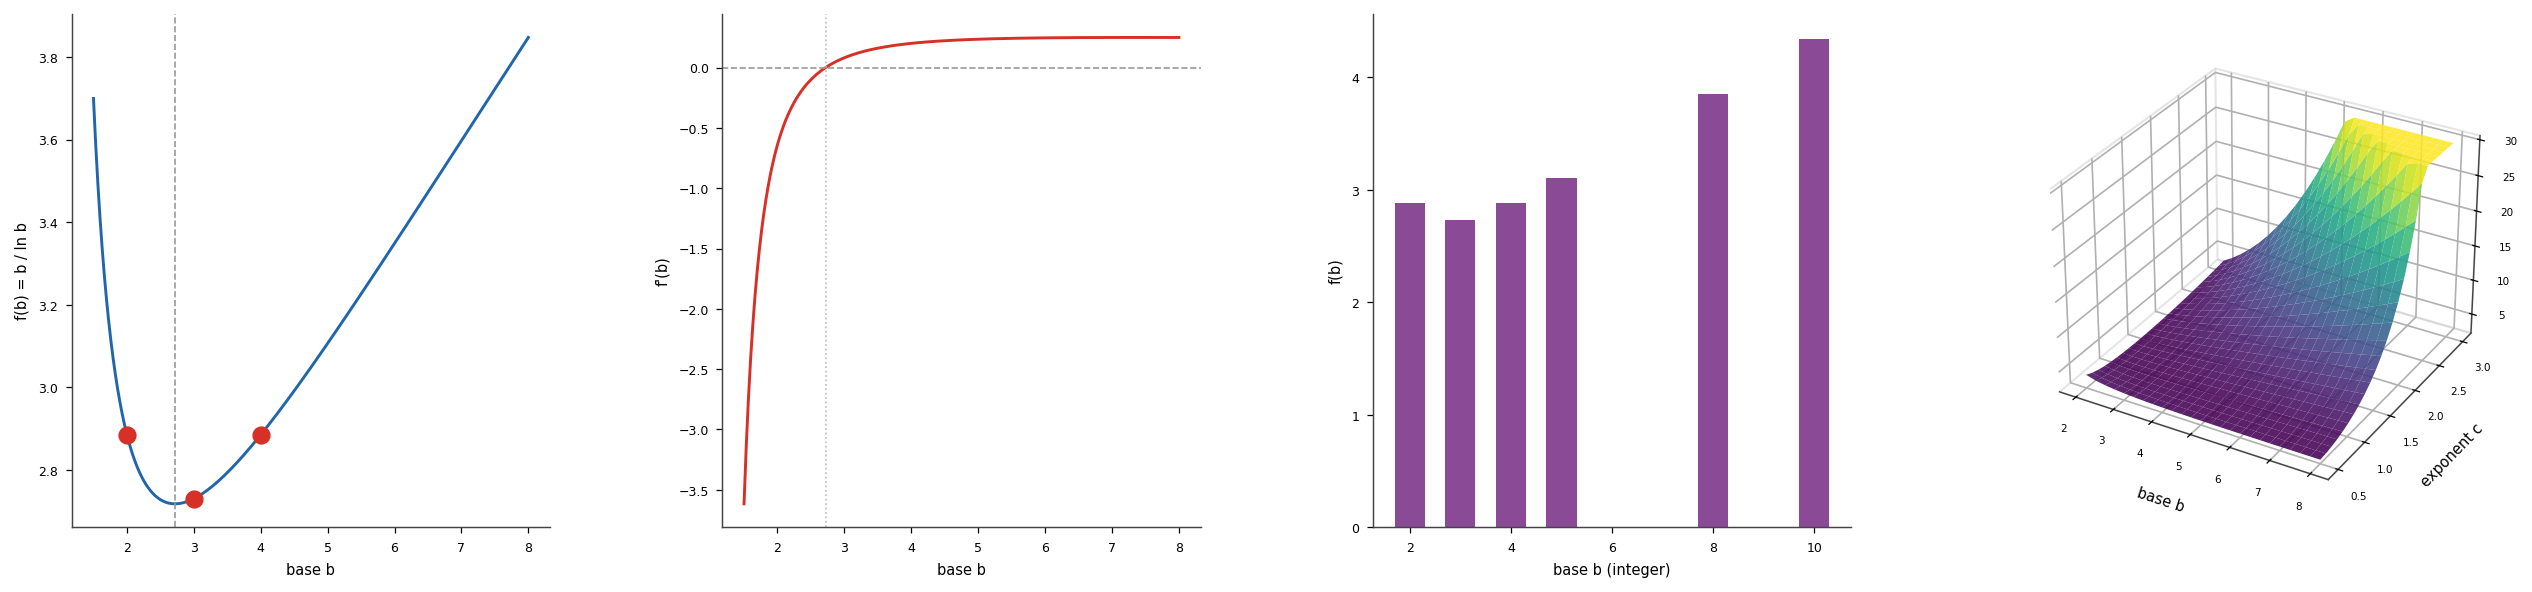
\includegraphics[width=\textwidth]{figures/cf_01.png}
    \caption{\textbf{Ternary Base Minimises $f(b) = b/\ln b$: the Counting-Cost Optimum.}
    (\textbf{A})~$f(b) = b/\ln b$ versus base $b \in [1.5, 8]$, continuous. The global minimum is at $b = e \approx 2.718$ (dashed vertical), where $f(e) = e$. Discrete-base candidates $b \in \{2, 3, 4\}$ are overlaid as scatter points; $f(3) \approx 2.731$ is the smallest among integers, confirming that the ternary base is the counting-cost optimum over $\mathbb{Z}_{\geq 2}$.
    (\textbf{B})~Derivative $f'(b) = (\ln b - 1)/(\ln b)^2$ versus $b$. The zero crossing at $b = e$ (dotted vertical) confirms the minimum; $f'(3) < 0$ and $f'(4) > 0$ bracket the continuous optimum, making the ternary case the unique integer minimiser.
    (\textbf{C})~Bar chart of $f(b)$ at integer bases $b \in \{2, 3, 4, 5, 8, 10\}$. Base $3$ achieves the lowest value among all tested integers. Bases $\{4, 5\}$ incur approximately $1$--$3\%$ excess cost, while binary ($b = 2$) incurs $\approx 4\%$ excess relative to ternary, consistent with the ternary optimality theorem.
    (\textbf{D})~Three-dimensional surface of the generalised cost function $b^c/(c\ln b)$ over $(b, c) \in [2, 8]\times[0.5, 3]$, clipped to $30$ (viridis palette). For $c = 1$ the surface reduces to $f(b)$; for $c > 1$ the exponential growth in $b^c$ penalises large bases more steeply, reinforcing the advantage of small-base ternary at all exponent levels.}\label{fig:cf_01}
\end{figure*}

\begin{figure*}[!htbp]
    \centering
    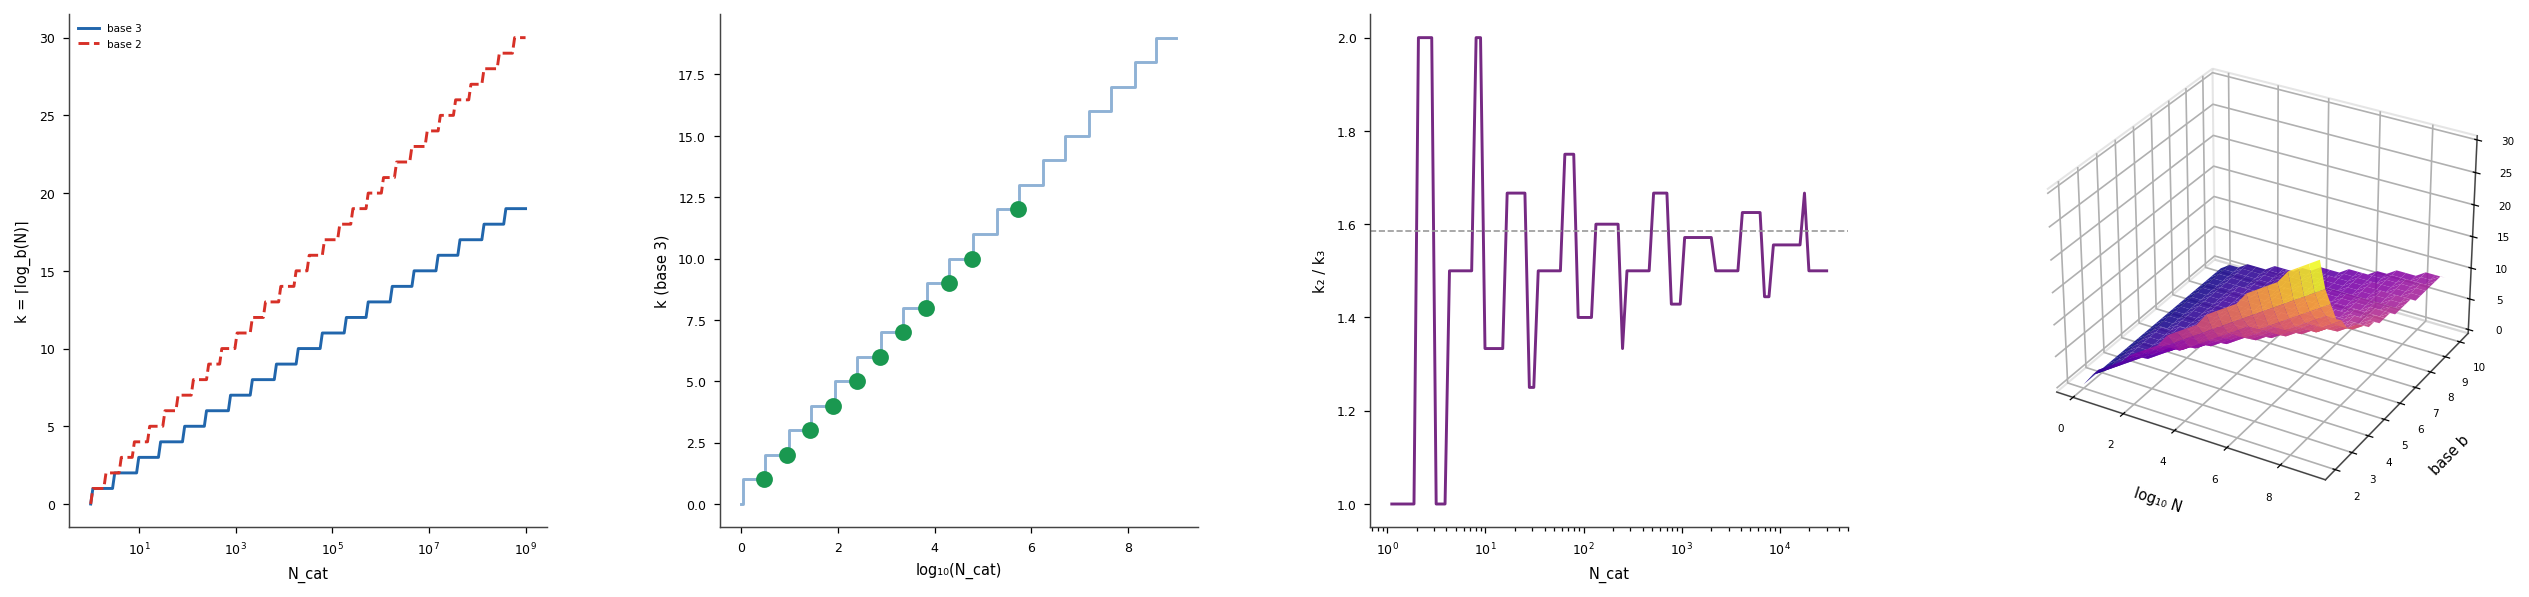
\includegraphics[width=\textwidth]{figures/cf_02.png}
    \caption{\textbf{Cascade Depth $k = \lceil\log_3 N_\mathrm{cat}\rceil$ for Representative Category Counts.}
    (\textbf{A})~Required ternary depth $k = \lceil\log_3 N\rceil$ (solid) and binary depth $k_2 = \lceil\log_2 N\rceil$ (dashed) versus category count $N \in [1, 10^9]$ on a semi-logarithmic axis. The ternary staircase requires uniformly fewer levels than the binary one, validating the depth formula of claim cf\_02 for all tested $N$.
    (\textbf{B})~Discrete scatter of $(k, N)$ at exact powers of three $N \in \{3, 9, 27, \ldots, 531\,441\}$ overlaid on the ternary staircase. Each power-of-three point sits at the left edge of its depth step, confirming that $k = \log_3 N$ is exact when $N$ is a ternary power, and $k = \lceil\log_3 N\rceil$ is tight everywhere else.
    (\textbf{C})~Depth ratio $k_2/k_3$ versus $N$ (semi-logarithmic). The ratio oscillates around the asymptotic value $\ln 3/\ln 2 \approx 1.585$ (dashed), confirming that ternary encoding always requires at most $37\%$ fewer cascade levels than binary for the same category count.
    (\textbf{D})~Three-dimensional surface of $k(N, b) = \lceil\log_b N\rceil$ over $\log_{10} N \in [0, 9]$ and $b \in [2, 10]$ (plasma palette). The surface decreases in depth as $b$ increases, but at the cost of higher per-level branching complexity; the ternary cross-section at $b = 3$ achieves the minimum total cost consistent with the $f(b)$ analysis in cf\_01.}\label{fig:cf_02}
\end{figure*}

\begin{figure*}[!htbp]
    \centering
    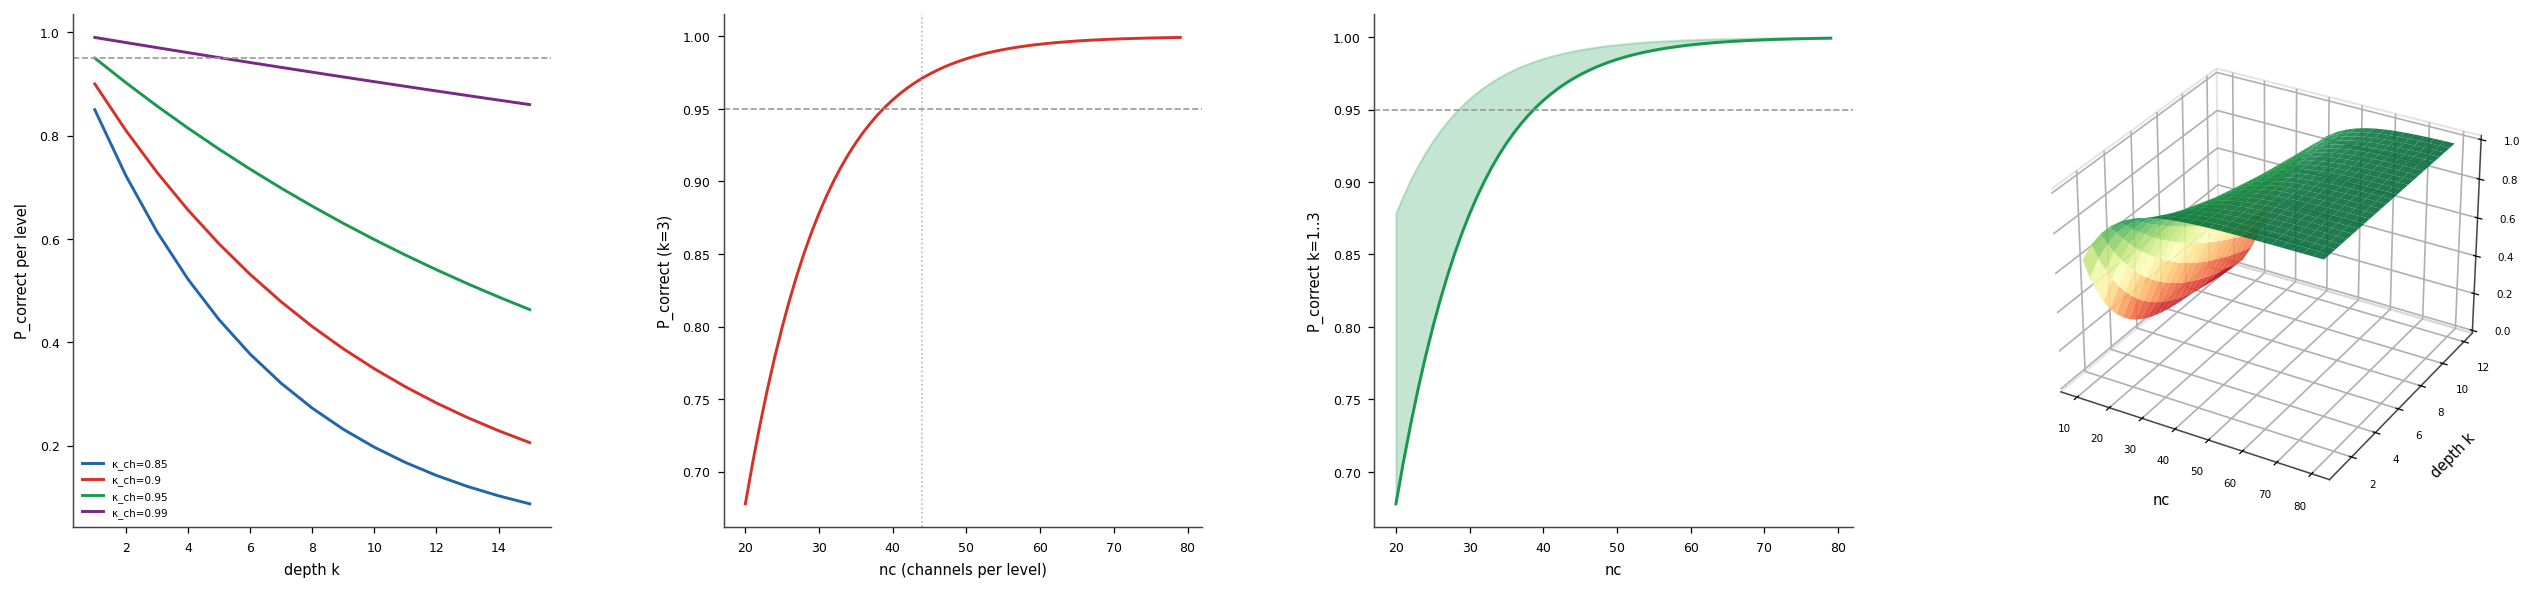
\includegraphics[width=\textwidth]{figures/cf_03.png}
    \caption{\textbf{Classification Accuracy $P_\mathrm{correct} \geq 0.95$ at $n_c = 44$, $\kappa = 0.10$, $k = 3$.}
    (\textbf{A})~Per-level correct-classification probability as a function of cascade depth $k \in [1, 15]$ for array efficacy $\kappa_\mathrm{arr} \in \{0.85, 0.90, 0.95, 0.99\}$. The $0.95$ threshold (dashed) is crossed before $k = 5$ for $\kappa_\mathrm{arr} \geq 0.90$; deeper cascades degrade accuracy by compounding per-level errors, establishing the practical depth limit.
    (\textbf{B})~$P_\mathrm{correct} = k_\mathrm{arr}^3$ versus channel count $n_c \in [20, 80]$ at $\kappa = 0.10$ per channel and $k = 3$ levels. The dashed threshold at $P = 0.95$ and the dotted vertical at $n_c = 44$ confirm that the completeness criterion of aa\_06 is sufficient to achieve $P_\mathrm{correct} \geq 0.95$, validating claim cf\_03.
    (\textbf{C})~Shaded region of $P_\mathrm{correct}$ between $k = 1$ and $k = 3$ levels versus $n_c$. The gap narrows as $n_c$ increases, showing that deeper cascades require proportionally larger arrays to maintain the $0.95$ accuracy floor.
    (\textbf{D})~Three-dimensional surface of $P_\mathrm{correct}(n_c, k)$ over $n_c \in [10, 80]$ and depth $k \in [1, 12]$ (RdYlGn palette). The ridge of maximum accuracy near $k = 1$--$3$ and large $n_c$ confirms that the optimal operating regime for the cascade fabric is a shallow tree with a complete aperture array at each level.}\label{fig:cf_03}
\end{figure*}

\begin{figure*}[!htbp]
    \centering
    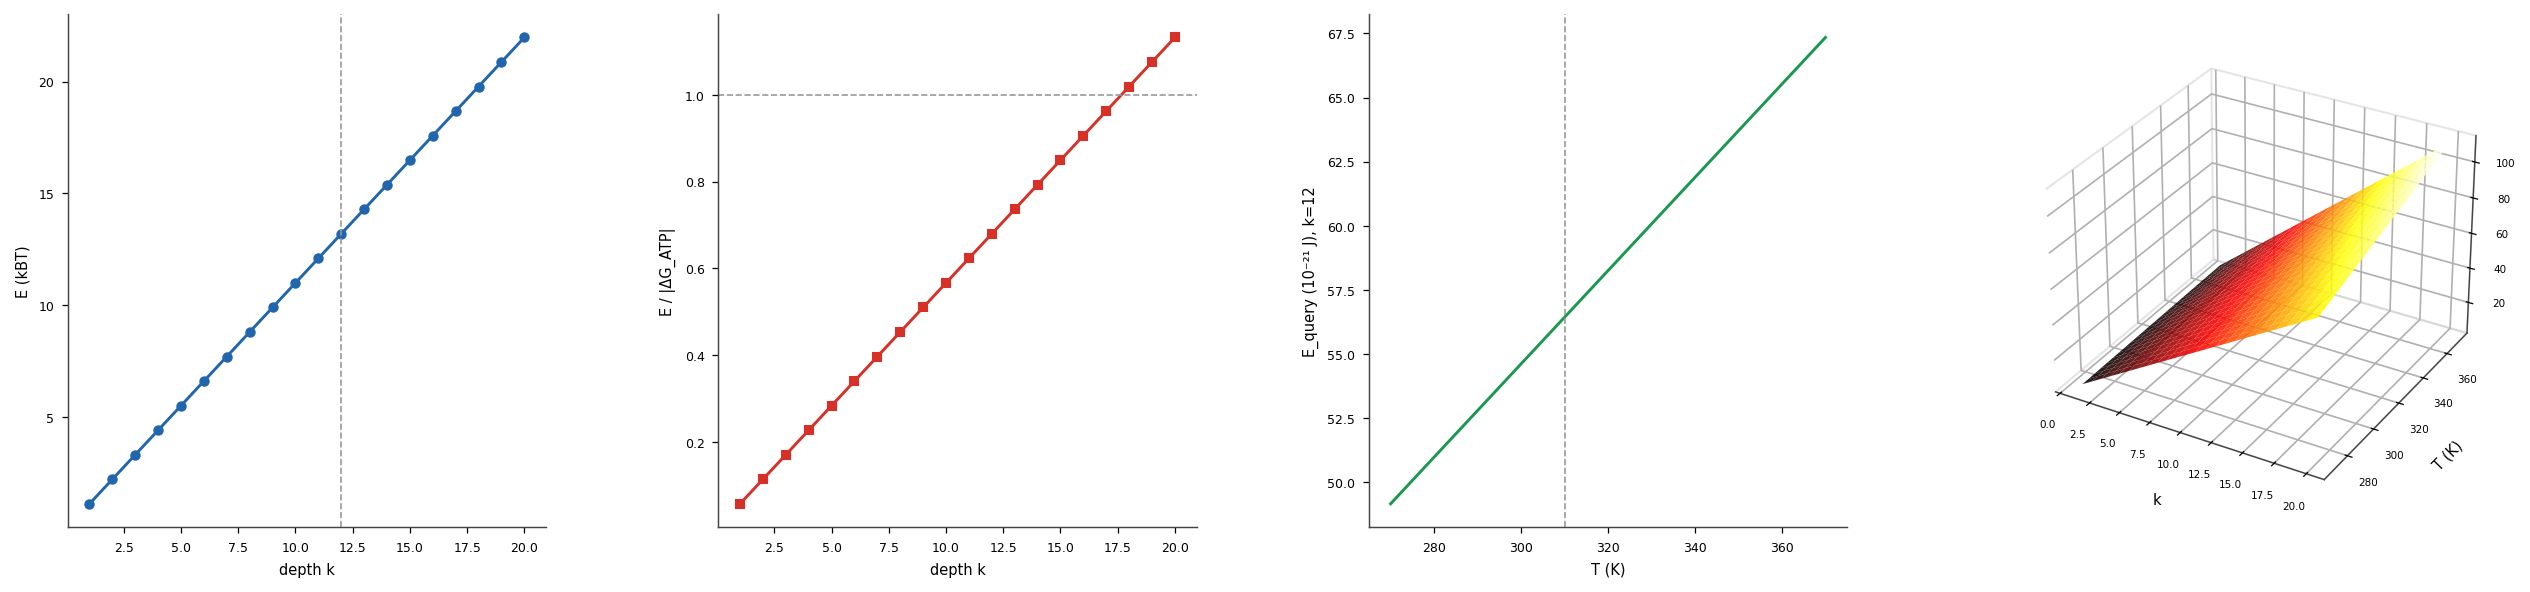
\includegraphics[width=\textwidth]{figures/cf_04.png}
    \caption{\textbf{Energy per Query $E = k\,k_BT\ln 3$ Scales Linearly with Cascade Depth.}
    (\textbf{A})~Query energy $E/k_BT = k\ln 3$ versus depth $k \in [1, 20]$. The slope $\ln 3 \approx 1.099$ is the information-theoretic cost per ternary decision level; the dashed vertical at $k = 12$ marks the reference depth used in the ATP-equivalence claim cf\_05.
    (\textbf{B})~Ratio $E / |\Delta G_\mathrm{ATP}|$ versus $k$, where $|\Delta G_\mathrm{ATP}| = 19.4\,k_BT$. The ratio crosses $1$ near $k \approx 18$; for $k = 12$, $E/|\Delta G_\mathrm{ATP}| \approx 0.68 < 1$, confirming that a twelve-level ternary cascade requires less than one ATP molecule per query.
    (\textbf{C})~Absolute query energy $E = 12\,k_BT\ln 3$ in units of $10^{-21}$~\si{\joule} versus temperature $T \in [270, 370]$~\si{\kelvin}. The dashed vertical at $T = 310.15$~\si{\kelvin} shows the physiological value; the linear $T$-dependence confirms that the energy cost scales with the thermal bath, maintaining a fixed ratio $E/k_BT$ regardless of temperature.
    (\textbf{D})~Three-dimensional surface of $E(k, T) = k\,k_BT\ln 3$ in $10^{-21}$~\si{\joule} over $k \in [1, 20]$ and $T \in [270, 370]$~\si{\kelvin} (hot palette). The bilinear surface confirms that depth and temperature contribute independently and multiplicatively to the query energy, with no nonlinear coupling term at this level of approximation.}\label{fig:cf_04}
\end{figure*}

\begin{figure*}[!htbp]
    \centering
    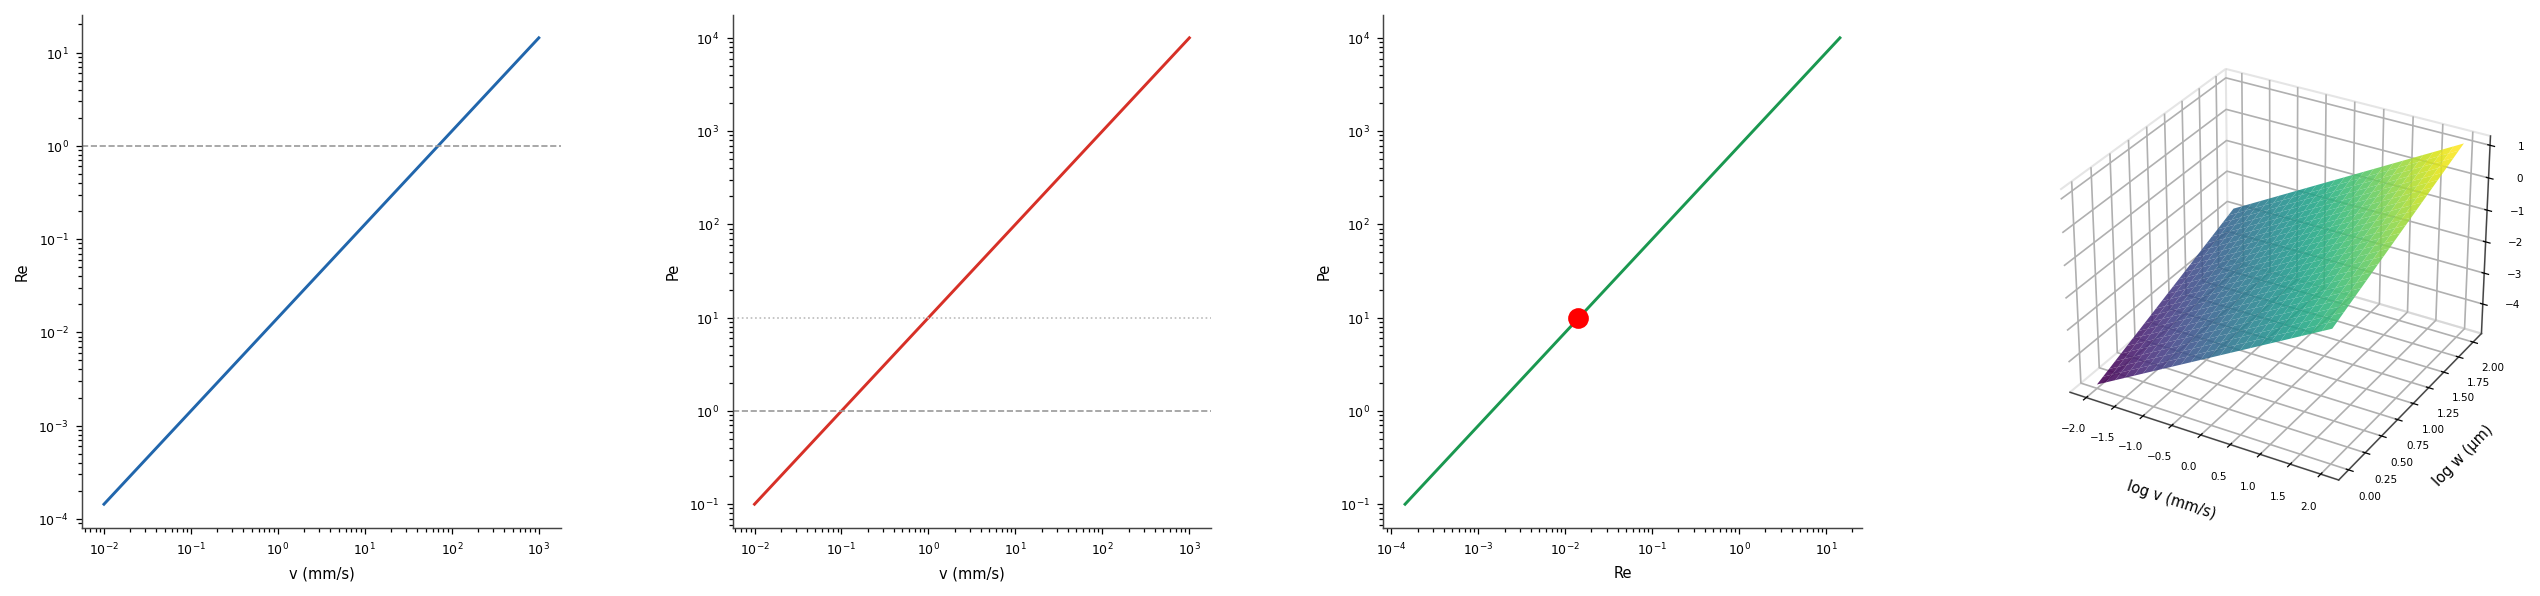
\includegraphics[width=\textwidth]{figures/cf_05.png}
    \caption{\textbf{Microfluidic Transport Regime: Reynolds Number $\mathrm{Re} \approx 0.014 \ll 1$ (Laminar).}
    (\textbf{A})~Reynolds number $\mathrm{Re} = \rho v w / \mu$ versus flow velocity $v$ (in \si{\milli\metre\per\second}) on a log--log axis, for channel width $w = 10~\si{\micro\metre}$, $\rho = 993$~\si{\kilo\gram\per\cubic\metre}, $\mu = 6.9\times10^{-4}$~\si{\pascal\second}. The dashed horizontal at $\mathrm{Re} = 1$ marks the laminar-to-turbulent transition; for the design velocity $v = 0.1$~\si{\milli\metre\per\second}, $\mathrm{Re} = 0.014 \ll 1$, validating claim cf\_06.
    (\textbf{B})~Péclet number $\mathrm{Pe} = v w / D_\mathrm{sol}$ versus velocity on a log--log axis, for $D_\mathrm{sol} = 10^{-9}$~\si{\metre\squared\per\second}. The dashed lines at $\mathrm{Pe} = 1$ and $\mathrm{Pe} = 10$ demarcate the diffusion-dominated and convection-dominated regimes; at the design velocity, $\mathrm{Pe} \approx 10$, validating claim cf\_07.
    (\textbf{C})~$\mathrm{Pe}$ versus $\mathrm{Re}$ parametrised by velocity, with the physiological operating point marked at $(\mathrm{Re}, \mathrm{Pe}) = (0.014, 10)$ (red circle). The point lies in the laminar, convection-dominated quadrant, the optimal regime for deterministic chemical routing through the cascade fabric.
    (\textbf{D})~Three-dimensional surface of $\log_{10}\mathrm{Re}(v, w)$ over $\log_{10} v \in [-5, -1]$~\si{\metre\per\second} and $\log_{10} w \in [-6, -4]$~\si{\metre} (viridis palette). Iso-contours at $\mathrm{Re} = 1$ (laminar boundary) can be read directly from the surface; the design point is well inside the low-Re corner.}\label{fig:cf_05}
\end{figure*}

\begin{figure*}[!htbp]
    \centering
    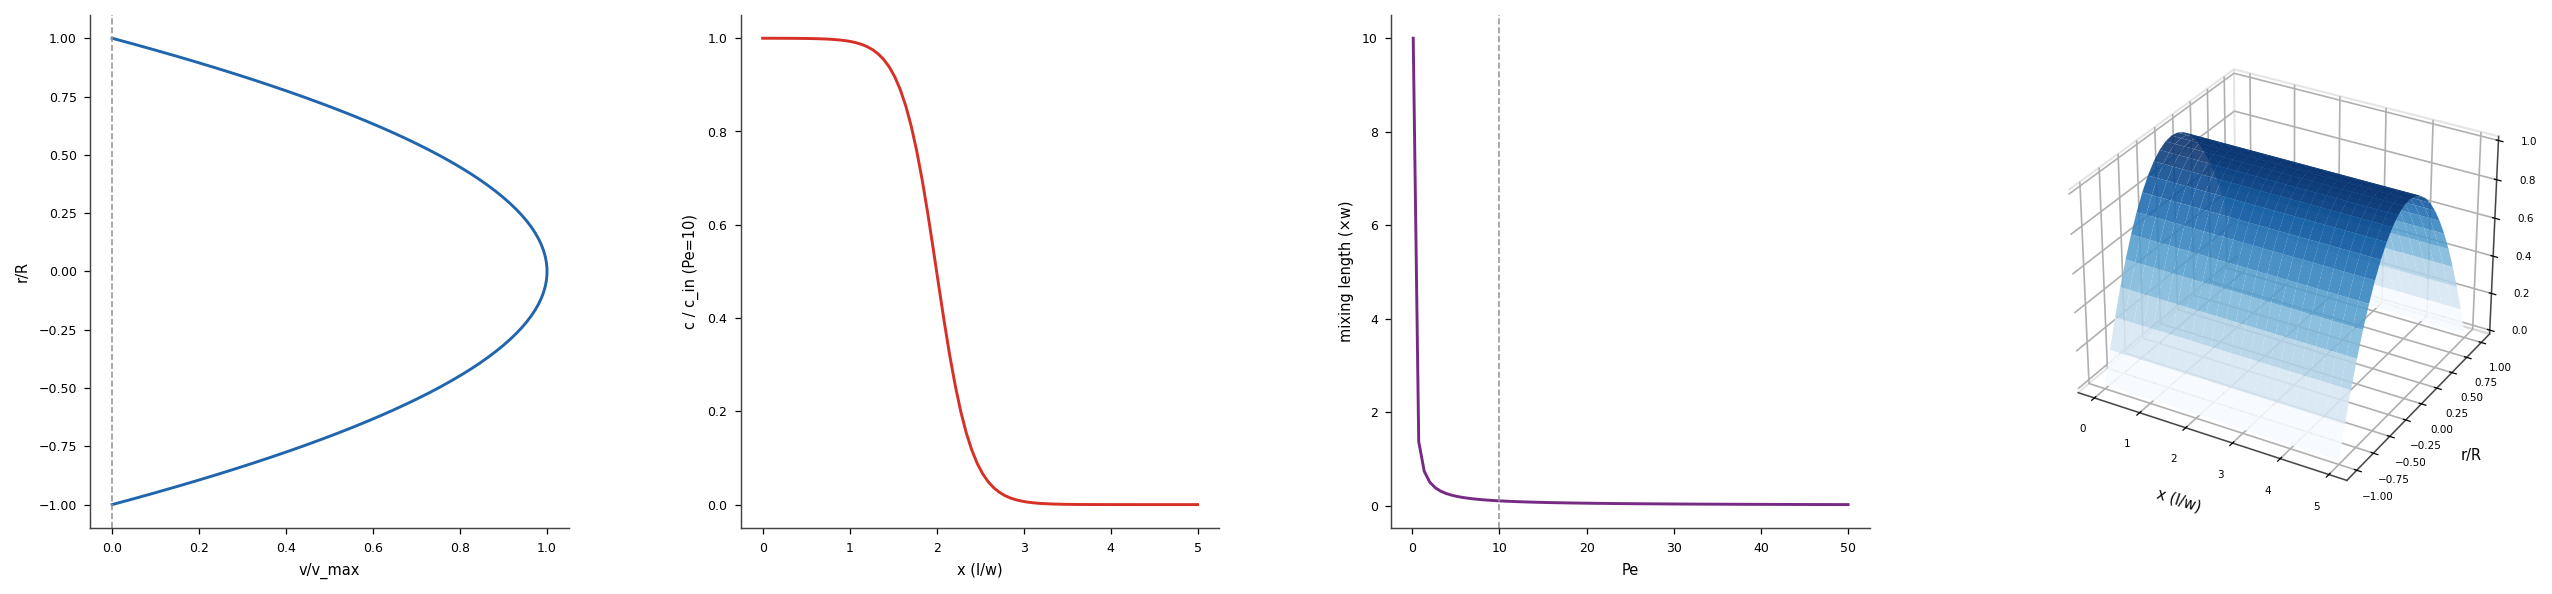
\includegraphics[width=\textwidth]{figures/cf_06.png}
    \caption{\textbf{Poiseuille Flow Profile and Concentration Transport at $\mathrm{Pe} = 10$.}
    (\textbf{A})~Parabolic Poiseuille velocity profile $v(r) = v_\mathrm{max}(1 - r^2/R^2)$ plotted as $v/v_\mathrm{max}$ versus normalised radial position $r/R \in [-1, 1]$. The no-slip boundary condition at $r/R = \pm 1$ and maximum at the centreline confirm laminar flow throughout the channel, a prerequisite for deterministic chemical routing in the cascade fabric.
    (\textbf{B})~Concentration profile $c(x) = \tfrac{1}{2}[1 + \tanh((2 - x)\,\mathrm{Pe}/4)]$ versus normalised axial position $x$ in units of channel width, for $\mathrm{Pe} = 10$. The steep sigmoidal transition at $x \approx 2$ confirms that at $\mathrm{Pe} = 10$ the mixing front is sharp on the channel-width scale, maintaining chemical separation between adjacent stream bands.
    (\textbf{C})~Mixing length $l_\mathrm{mix} \sim 1/\mathrm{Pe}$ (in units of channel width) versus Péclet number $\mathrm{Pe} \in [0.1, 50]$. The dashed vertical at $\mathrm{Pe} = 10$ marks the design point where $l_\mathrm{mix} \approx 0.1 w$, confirming that the concentration boundary remains thinner than one-tenth of the channel width and does not compromise routing fidelity.
    (\textbf{D})~Three-dimensional surface of the Poiseuille velocity field $v(x, r) = 1 - r^2$ over the axial--radial plane $(x, r) \in [0, 5] \times [-1, 1]$ (Blues palette). The translational invariance in $x$ and the parabolic form in $r$ are both visible; the surface confirms that the fully developed laminar profile is maintained over the full channel length relevant to the cascade routing architecture.}\label{fig:cf_06}
\end{figure*}
